
\documentclass[a4paper, 10pt,  conference]{article}  

\usepackage{geometry}
\geometry{legalpaper, margin=1in}
    
    
\usepackage{verbatim}
\usepackage{graphicx}
\usepackage{pdfpages}
\usepackage{cite}


\setlength{\parskip}{1em}



\title{\LARGE \bf FESTO Project 2\\Mechatronics 282 778}
\author{Marc Alexander Sferrazza
\thanks{This work was not supported by any organization}
\thanks{Faculty of Mechatronics Engineering, Massey University, Albany, Auckland, New Zealand
        {\tt\small Progress of project: https://github.com/alex1v1a/Mechatronics/tree/master/Project\%202} } }

\begin{document}

\maketitle

\begin{figure}[h!]
  
\includegraphics[width=\linewidth]{images/FESTO-Logo}
  \label{fig:FESTO-Logo}
\end{figure}

\thispagestyle{empty}
\pagestyle{empty}


%%%%%%%%%%%%%%%%%%%%%%%%%%%%%%%%%%%%%%%%%%%%%%%%%%%%%%%%%%%%%%%%%%%%%%%%%%%%%%%%

\begin{abstract}

A brief report on Festo PLC programming and the process for four module stations. Each station was tested and debugged to ensure a robust result with exception of station 3 which has been coded in theory but not tested as the station is disabled.

\end{abstract}


\clearpage
\tableofcontents
\clearpage

%%%%%%%%%%%%%%%%%%%%%%%%%%%%%%%%%%%%%%%%%%%%%%%%%%%%%%%%%%%%%%%%%%%%%%%%%%%%%%%%
%%%%%%%%%%%%%%%%%%%%%%%%%%%%%%%%%%%%%%%%%%%%%%%%%%%%%%%%%%%%%%%%%%%%%%%%%%%%%%%%


\section{INTRODUCTION}
To design the manufacturing based tasked of the Festo MPS (modular production system) stations using PLC (programmable logic controller) programming. When considering control of the modular stations a series of sensors and actuators of mechanical, pneumatic and electrical are revised. There are 4 stations of which each contain specific sorting tasks that utilise the range of many interconnected relays to preform sequential logical instructions in loops stored locally on the device. Utilising these gates instructions will be given to move an array of pucks from point A to point B while simultaneously sorting them in some cases.



%%%%%%%%%%%%%%%%%%%%%%%%%%%%%%%%%%%%%%%%%%%%%%%%%%%%%%%%%%%%%%%%%%%%%%%%%%%%%%%%
%%%%%%%%%%%%%%%%%%%%%%%%%%%%%%%%%%%%%%%%%%%%%%%%%%%%%%%%%%%%%%%%%%%%%%%%%%%%%%%%

\section{METHOD}
Template files given for the allocation list, default Stop and Emergency programs are used with the project to replicate a given instruction produced in the provided videos for each module station.


%%%%%%%%%%%%%%%%%%%%%%%%%%%%%%%%%%%%%%%%%%%%%%%%%%%%%%%%%%%%%%%%%%%%%%%%%%%%%%%%

\subsection{Programming the PLC}
Using the statement method an instruction has been written to control the PLC system. There is also another method using a graphical map of ladder logic; however due to the simplicity of the STEP function the statement method has been chosen for easy to follow logical steps.


%%%%%%%%%%%%%%%%%%%%%%%%%%%%%%%%%%%%%%%%%%%%%%%%%%%%%%%%%%%%%%%%%%%%%%%%%%%%%%%%

\subsection{Algorithm}
For every station a set of initialisation commands are given for when the user selects input, start, stop or reset while manual switch is on. The start operation sets the station to initial position then preforms the sequence tasks as instructed by steps. The stop operation immediately seizes all functions and brings the system to a halt, while the reset button will return the all functions to initial positions and reset the entire system at any time.


%%%%%%%%%%%%%%%%%%%%%%%%%%%%%%%%%%%%%%%%%%%%%%%%%%%%%%%%%%%%%%%%%%%%%%%%%%%%%%%%

\subsection{Station One}




%%%%%%%%%%%%%%%%%%%%%%%%%%%%%%%%%%%%%%%%%%%%%%%%%%%%%%%%%%%%%%%%%%%%%%%%%%%%%%%%

\subsection{Station two}




%%%%%%%%%%%%%%%%%%%%%%%%%%%%%%%%%%%%%%%%%%%%%%%%%%%%%%%%%%%%%%%%%%%%%%%%%%%%%%%%

\subsection{Station three}




%%%%%%%%%%%%%%%%%%%%%%%%%%%%%%%%%%%%%%%%%%%%%%%%%%%%%%%%%%%%%%%%%%%%%%%%%%%%%%%%

\subsection{Station four}





%%%%%%%%%%%%%%%%%%%%%%%%%%%%%%%%%%%%%%%%%%%%%%%%%%%%%%%%%%%%%%%%%%%%%%%%%%%%%%%%
%%%%%%%%%%%%%%%%%%%%%%%%%%%%%%%%%%%%%%%%%%%%%%%%%%%%%%%%%%%%%%%%%%%%%%%%%%%%%%%%


\section{RESULTS}
Completing tasks for programming each of the stations and linking them together in a series to provide an efficient step by step system as displayed per each demonstration video. Each task was completed and checked for errors in runtime with physical testing for a robust program outside of the videos demonstration. Stages on what to do after  the tasks have been completed, before the task starts, what to do in result of a malfunction and linking the stations together have all been completed in the steps below. The entire programming task for all stations took 6-8 solid hours to learn and write, which felt significantly less due to the deep focus at the time. This was not that demanding in time but did require some thought effort to realise what stages things can work, but after the initial logic was realised, the rest of the program was simple.


%%%%%%%%%%%%%%%%%%%%%%%%%%%%%%%%%%%%%%%%%%%%%%%%%%%%%%%%%%%%%%%%%%%%%%%%%%%%%%%%

\subsection{Debugging} 
While the process is straight forward and consists of step by step operations, the procedure in which to get there is not. While in a program a system may appear sound, there are many underlying issues, that of which if are not addressed will cause serious malfunction down the line. 

It is imperative that all processes are enabled and disabled in a suitable fashion such that the system is reliant on the next steps status. This means that while it may be simple to just use a timer and guess the time intervals between stages, after the 10th or 100th or 1000th step the time interval may have adjusted out of sync with the rest of the sequence and thus cause a jam, or other malfunction in which is catastrophic for the system. To avoid this simple stages based on sensors are used in steps, and timers may be used in these steps as long as such use is consistent with the stages in the loop and will not potentially become out of phase with the system.

%%%%%%%%%%%%%%%%%%%%%%%%%%%%%%%%%%%%%%%%%%%%%%%%%%%%%%%%%%%%%%%%%%%%%%%%%%%%%%%%

\subsection{Testing}
It is always important to test the system for any glitches while debugging. There is always room for improvement in making the system more efficient and effective from start to finish. This includes ensuring that the system knows what to do in the event that the task at hand is complete, or even after this stage when more tasks or jobs are added to the system.

The Festo program also offers live debugging with current status of steps with the online function. While I did not find this particularly useful as I did not need to use it; I did however explore this procedure which displays live feedback for the status of sensors throughout the steps of the system.


%%%%%%%%%%%%%%%%%%%%%%%%%%%%%%%%%%%%%%%%%%%%%%%%%%%%%%%%%%%%%%%%%%%%%%%%%%%%%%%%

\subsection{Finalising}
Making the system stable and concise with as few steps, and as robust as possible builds for a good design. The method of testing all variables that might effect the system is required to make this achievable. 


%%%%%%%%%%%%%%%%%%%%%%%%%%%%%%%%%%%%%%%%%%%%%%%%%%%%%%%%%%%%%%%%%%%%%%%%%%%%%%%%
%%%%%%%%%%%%%%%%%%%%%%%%%%%%%%%%%%%%%%%%%%%%%%%%%%%%%%%%%%%%%%%%%%%%%%%%%%%%%%%%


\section{CONCLUSIONS}
The procedure of breaking a system down into steps and stages to build up a process cain of stable instructions is relatively straight forward, and easy enough of language to understand for the next person to come along and recognise what is happening. It is very well structured and being able to debug a complex set of sequences and tweak with very little difficulty. The immediate advantages of the direct response to sensors and actuation makes for a great way to preform any set of tasks by instigating a signals high or low outputs to preform a task in correct order with very low room for fault rate.

PLC is an easy to learn language with great potential and versatility in a range of manufacturing lines, and is used in many industries today. While expensive to prototype, once in place the system is robust and efficient saving costs in the long term if maintained and set up correctly.


%%%%%%%%%%%%%%%%%%%%%%%%%%%%%%%%%%%%%%%%%%%%%%%%%%%%%%%%%%%%%%%%%%%%%%%%%%%%%%%%
%%%%%%%%%%%%%%%%%%%%%%%%%%%%%%%%%%%%%%%%%%%%%%%%%%%%%%%%%%%%%%%%%%%%%%%%%%%%%%%%

\clearpage
\nocite{*}
\nocite{key}
\bibliographystyle{ieeetr}
\bibliography{references}

%%%%%%%%%%%%%%%%%%%%%%%%%%%%%%%%%%%%%%%%%%%%%%%%%%%%%%%%%%%%%%%%%%%%%%%%%%%%%%%%
%%%%%%%%%%%%%%%%%%%%%%%%%%%%%%%%%%%%%%%%%%%%%%%%%%%%%%%%%%%%%%%%%%%%%%%%%%%%%%%%

\clearpage
\section*{APPENDIX}

\begin{figure}[h!]
  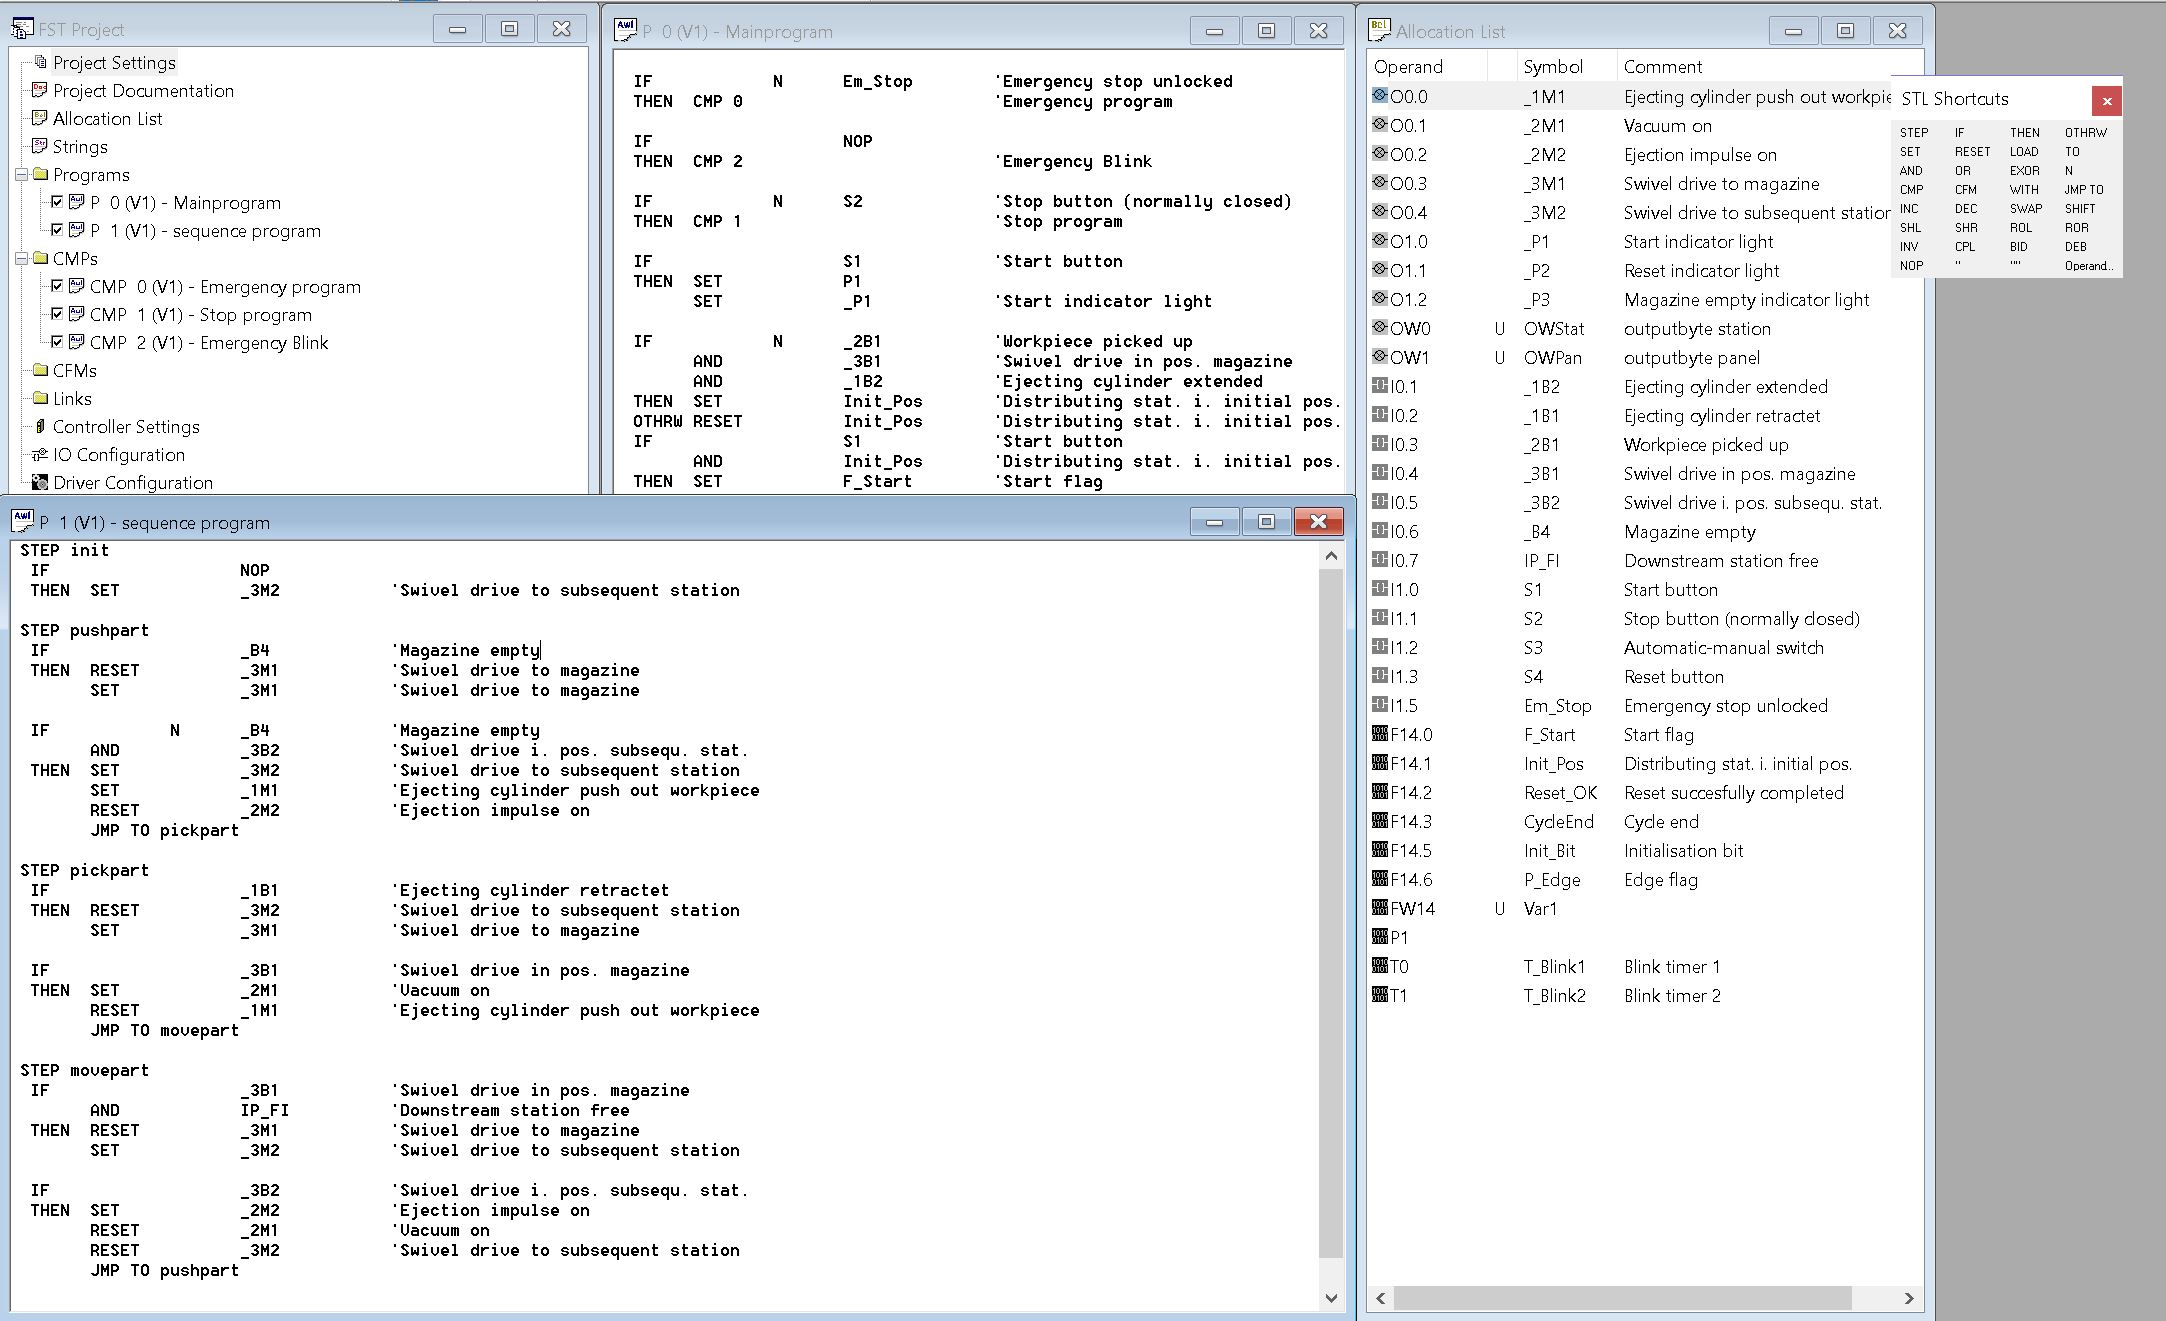
\includegraphics[width=\linewidth]{images/1}
  \caption{Station 1}
  \label{fig:Station 1}
\end{figure}

\begin{figure}[h!]
  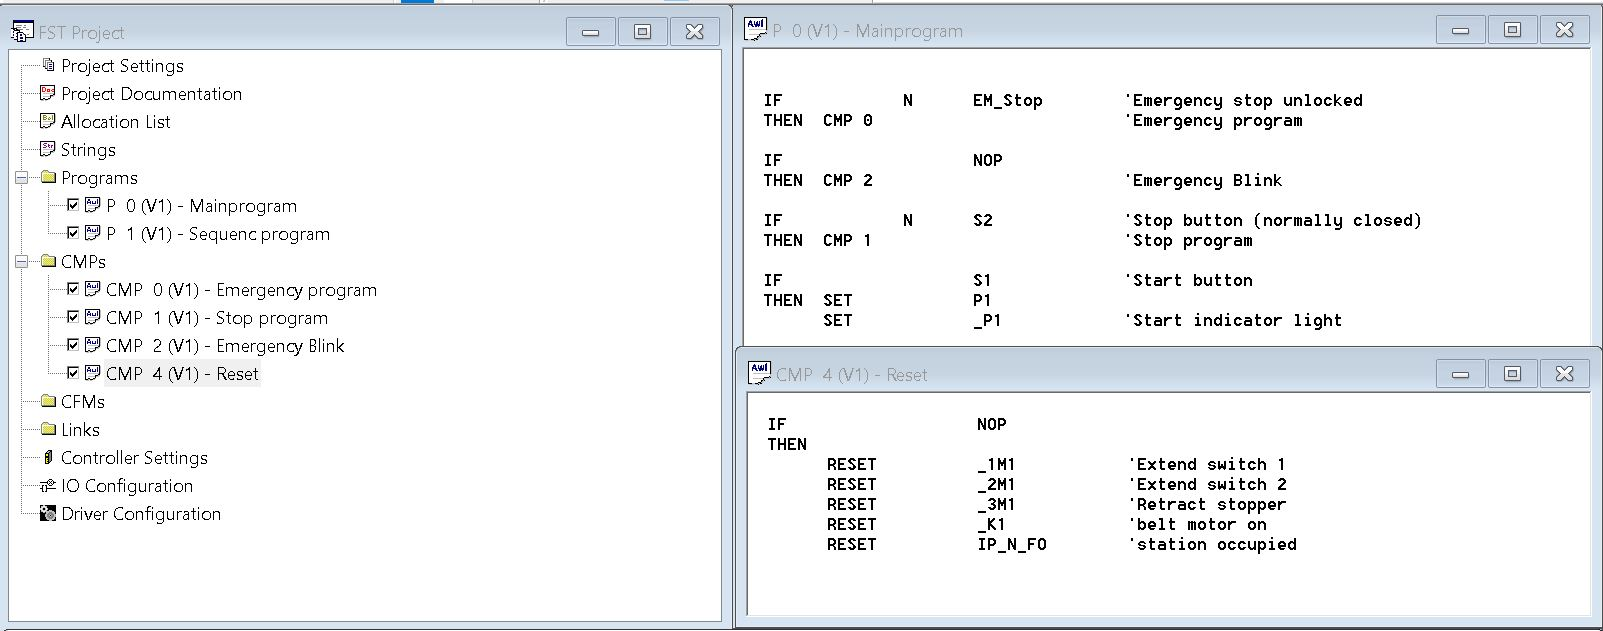
\includegraphics[width=\linewidth]{images/2}
  \caption{Station 2}
  \label{fig:Station 2}
\end{figure}

\begin{figure}[h!]
  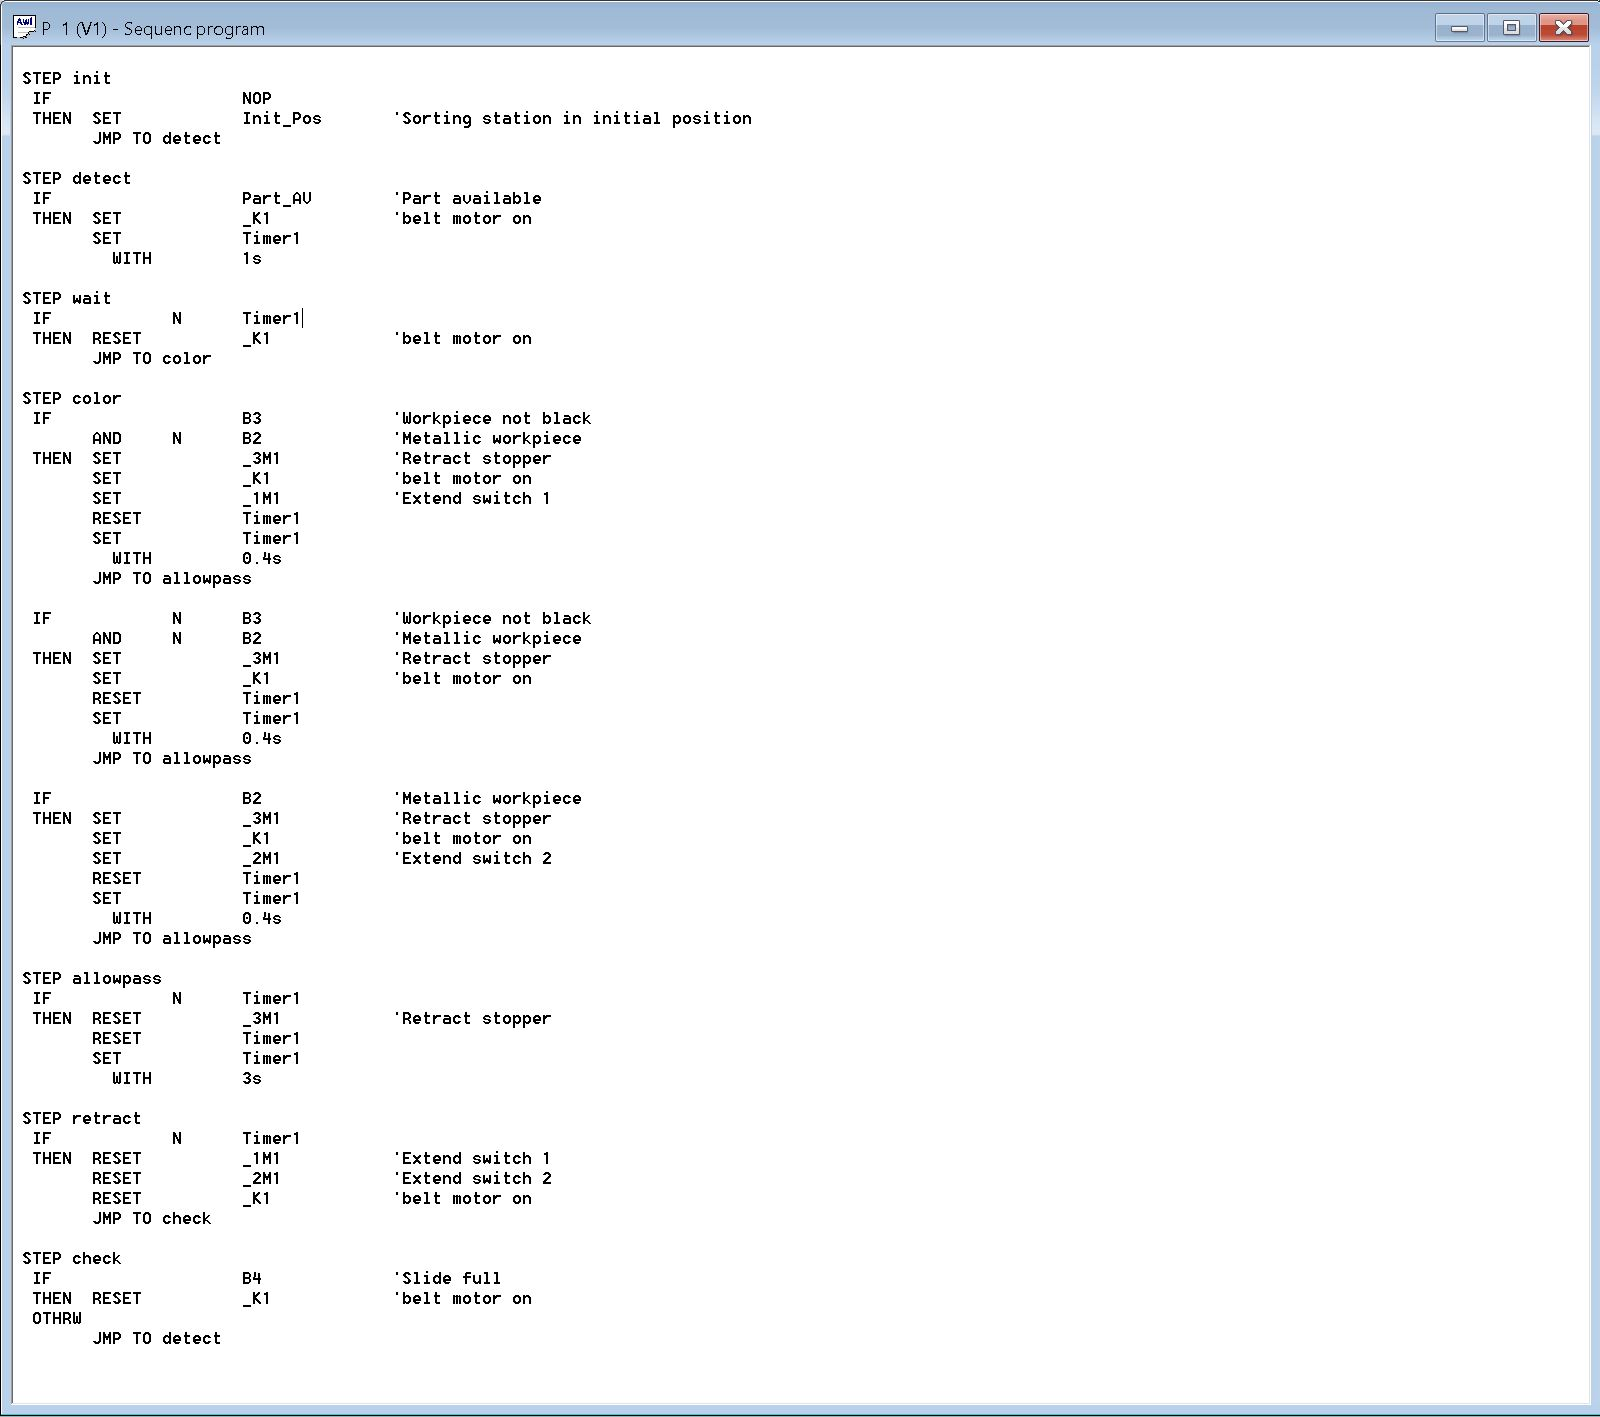
\includegraphics[width=\linewidth]{images/21}
  \caption{Station 2 Sequence}
  \label{fig:Station 2}
\end{figure}

\begin{figure}[h!]
  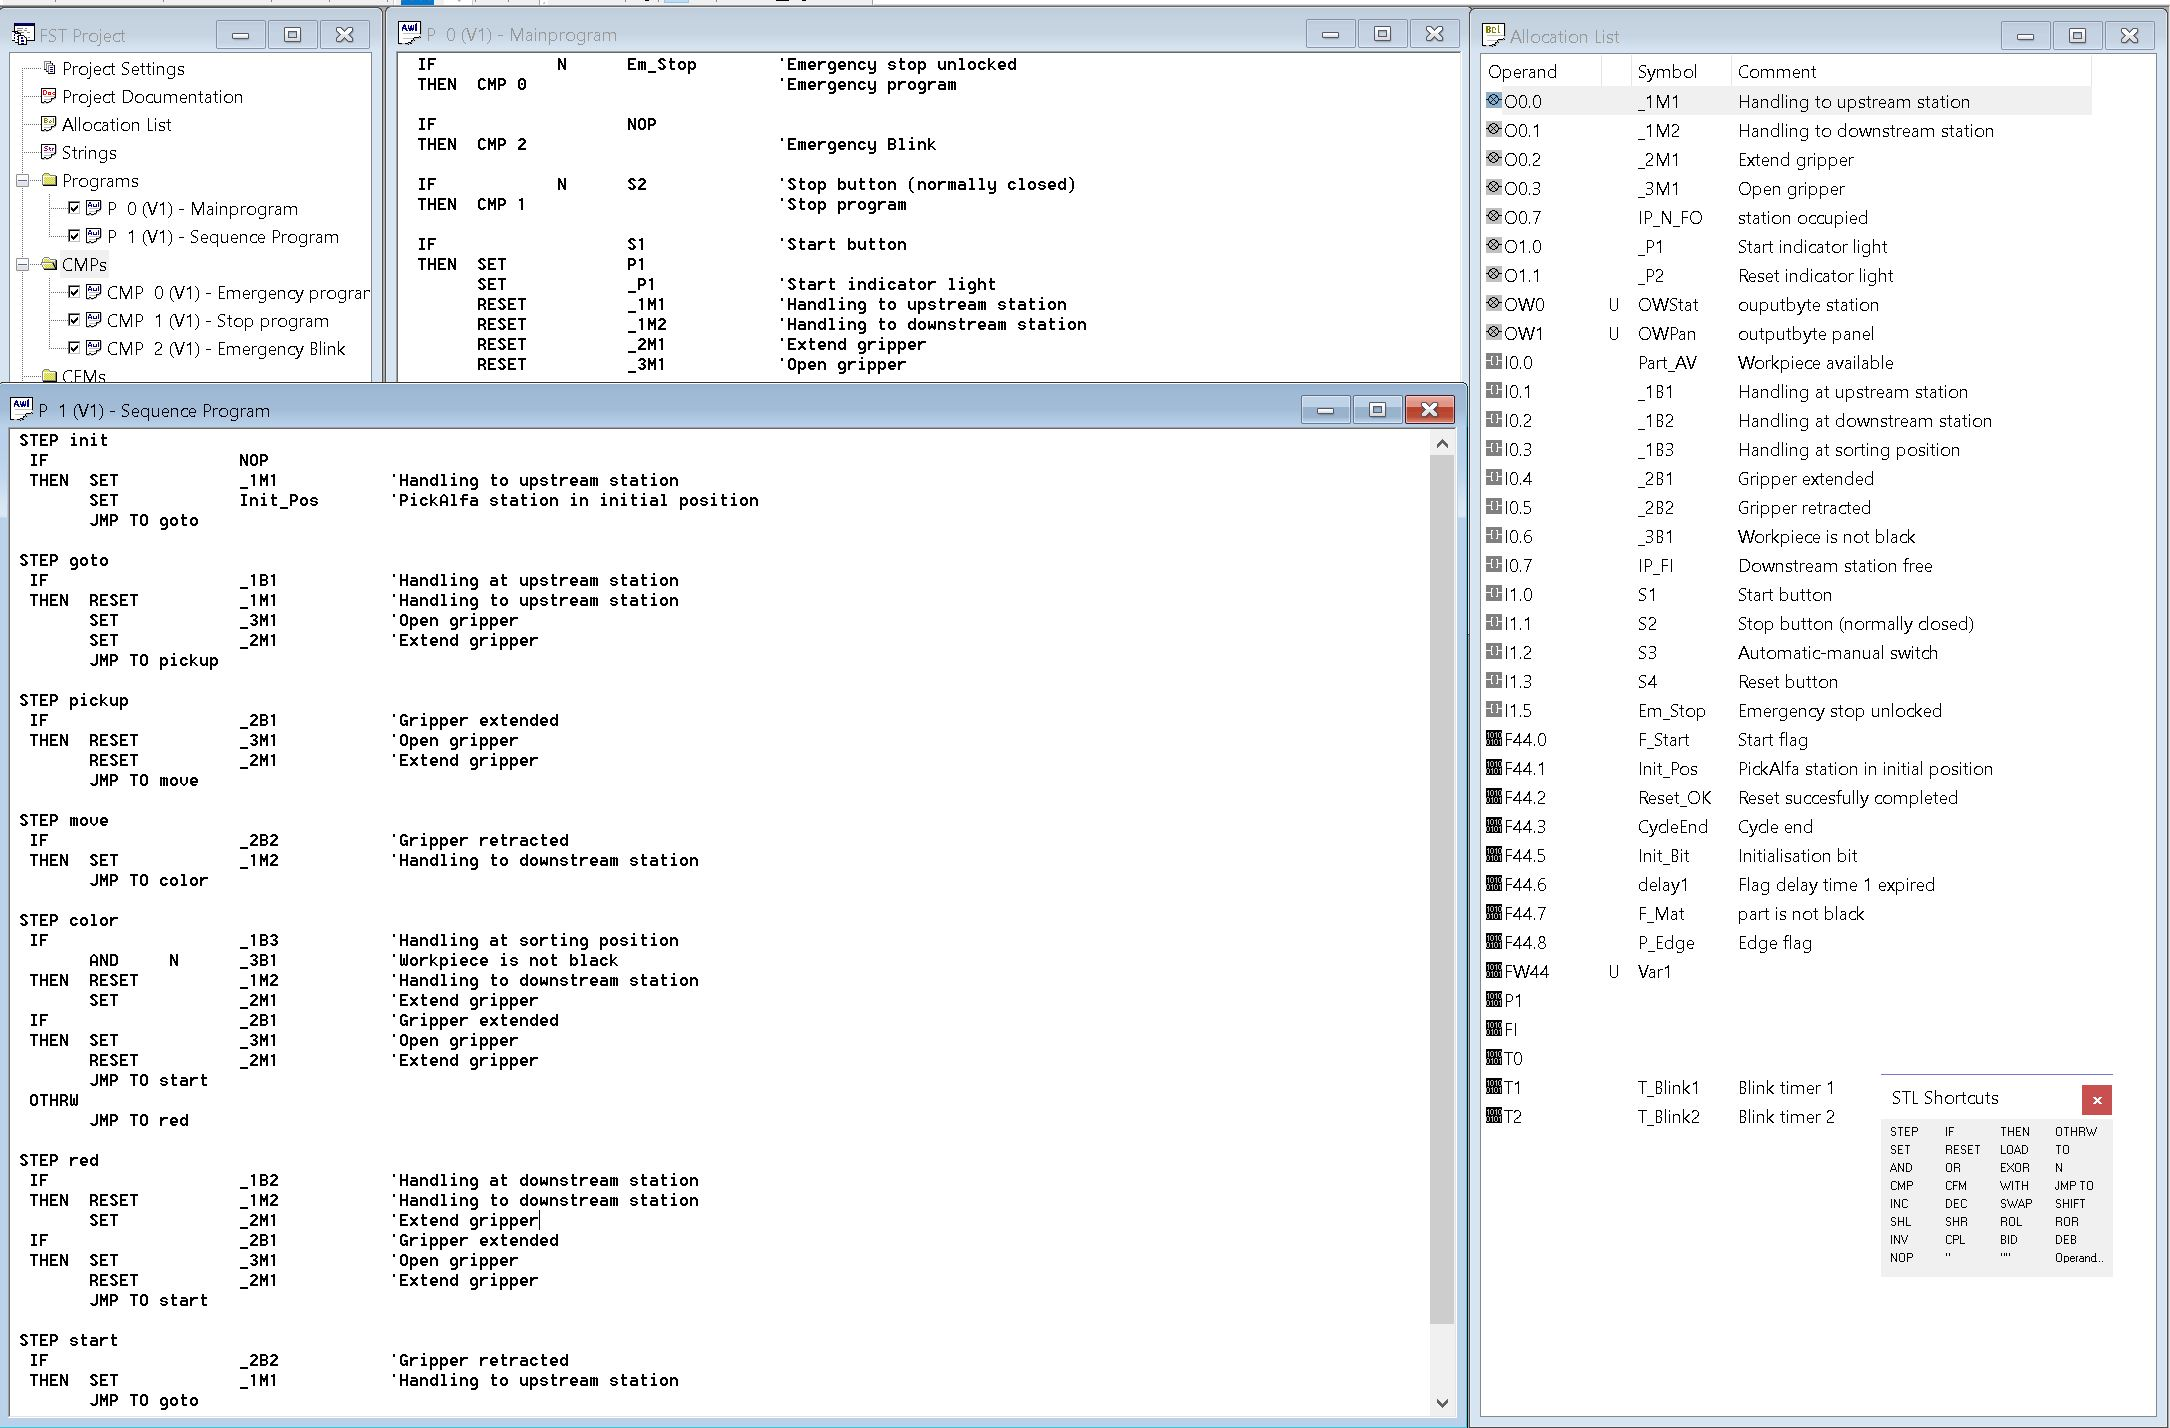
\includegraphics[width=\linewidth]{images/3}
  \caption{Station 3}
  \label{fig:Station 3}
\end{figure}

\begin{figure}[h!]
  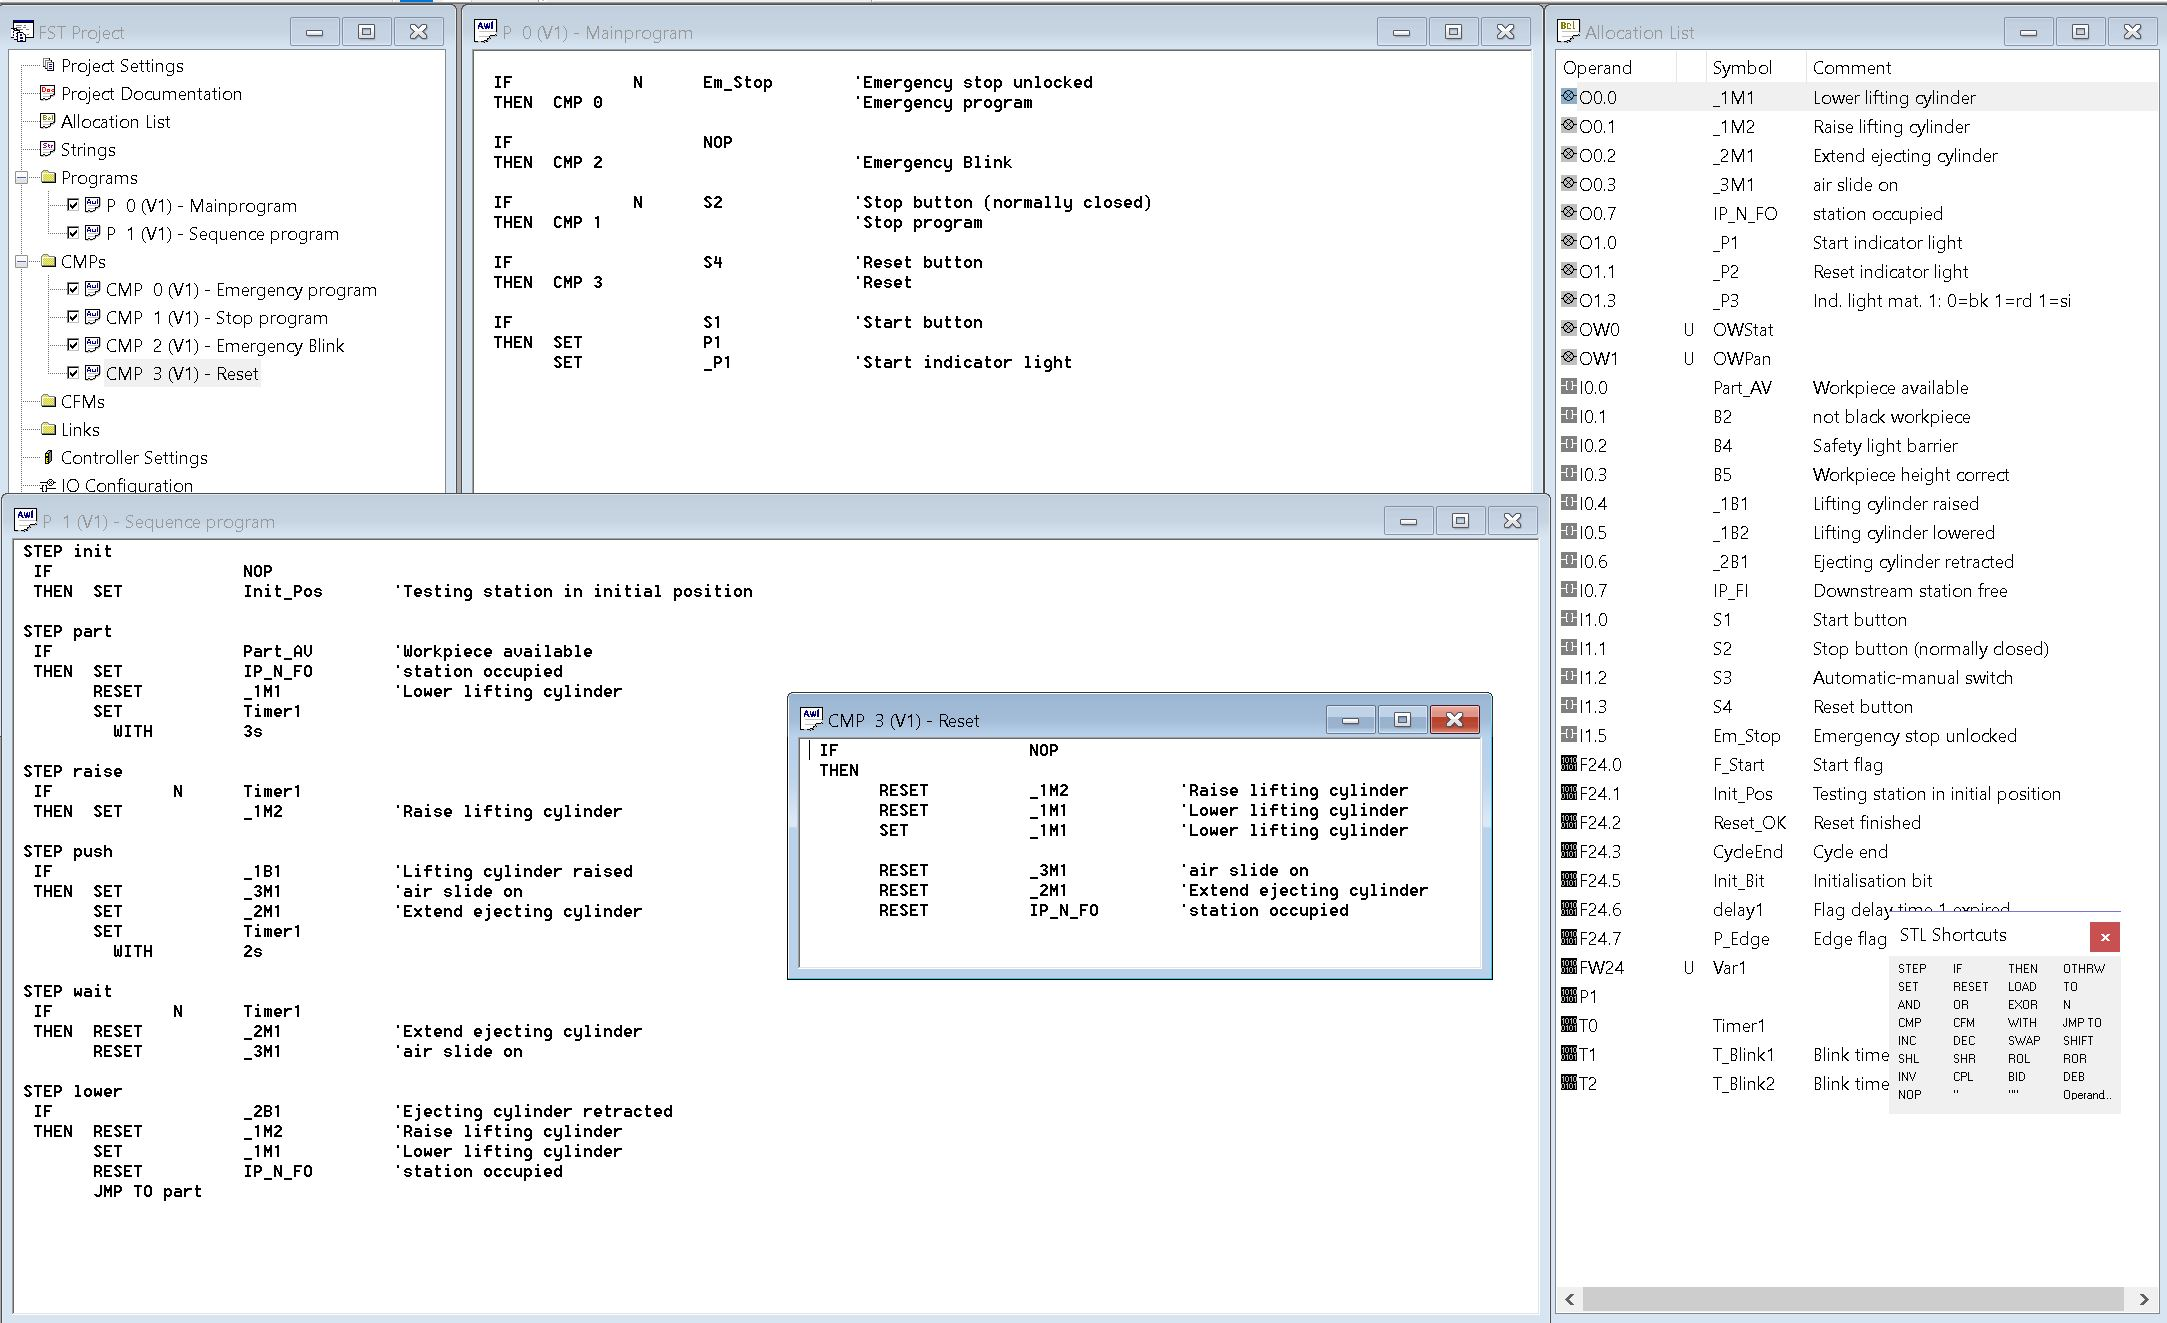
\includegraphics[width=\linewidth]{images/4}
  \caption{Station 4}
  \label{fig:Station 4}
\end{figure}



\end{document}
